\appendix

\chapter {Calculations}

\section {Minimum UART speed calculation}

Given 2 sensors and a time resolution of 10ms (refer to Figure 4.9),

\begin{equation}
\frac{10\ ms}{12\ parts} \div 4\ parts = 4800\ Hz
\end{equation}
\begin{equation}
\frac {4800} {s} \times 16\ bits = 76\ 800\ bit/s
\end{equation}

\section {DPF calculation}

The differential path length factor (DPF) can be calculated from the following equation \cite{rosen05}

\begin{equation}
DPF^\lambda = \frac{1}{2}\left(\frac{3\mu_{s}^\lambda}{\mu_{a}^\lambda}\right)^{1/2} \left(1-\frac{1}{1+d(3\mu_{s}^\lambda\mu_{a}^\lambda)^{1/2}}\right)
\end{equation}

The absorption ($\mu_{a}^\lambda$) and reduced scattering ($\mu_{s}^\lambda$) coefficients cannot be directly measured by near infrared light, so the values given in past studies will be used. Specifically, $\mu_{a}^{730nm}$=0.015 mm$^{-1}$, $\mu_{a}^{850nm}$ = 0.023 mm$^{-1}$, $\mu_{s}^{730nm}$= 0.80 mm$^{-1}$, and $\mu_{s}^{850nm}$=0.95 mm$^{-1}$. The values at 750nm could not be found, so the values at 730nm will be used. Plugging these values into the equation above gives, $DPF^{730nm}$=5.0055 and $DPF^{850nm}$=4.6564.

\chapter{Flow Charts}
\section {Microcontroller code flow chart}

\headsep = 5pt
\begin{figure}[htp]
\centering
\caption{Microcontroller code flow chart}
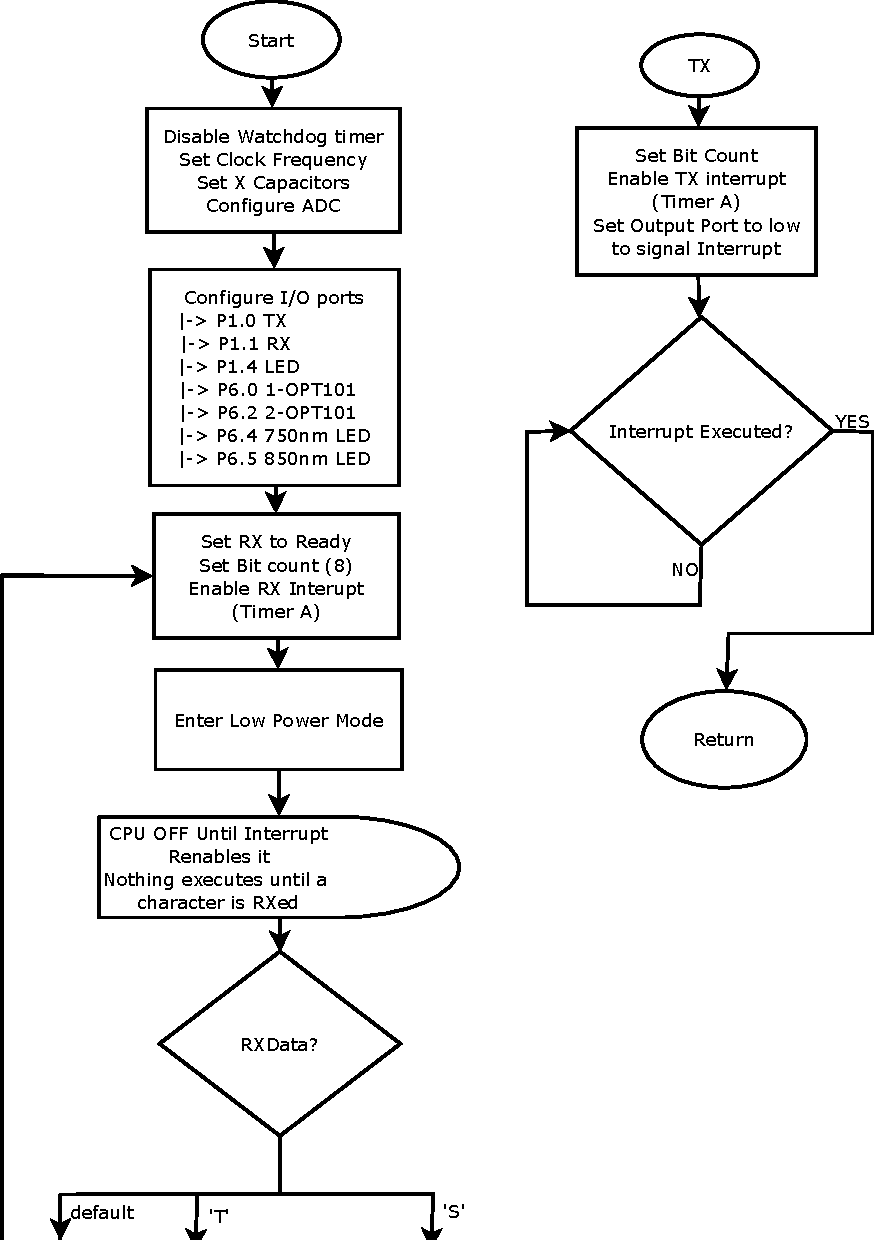
\includegraphics[height=8.05in]{cdia-1.pdf}
\end{figure}

\begin{figure}[htp]
\centering
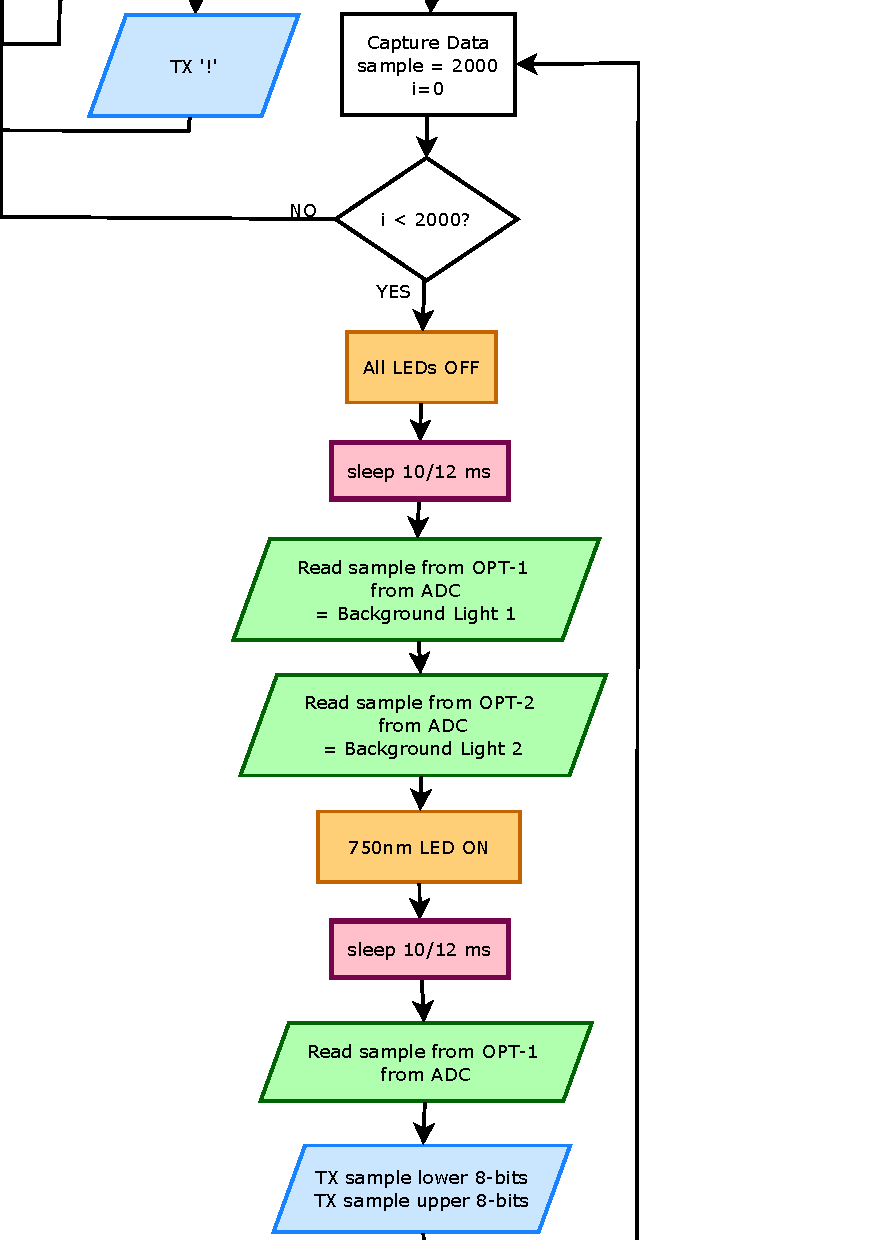
\includegraphics{cdia-2.pdf}
\end{figure}

\begin{figure}[htp]
\centering
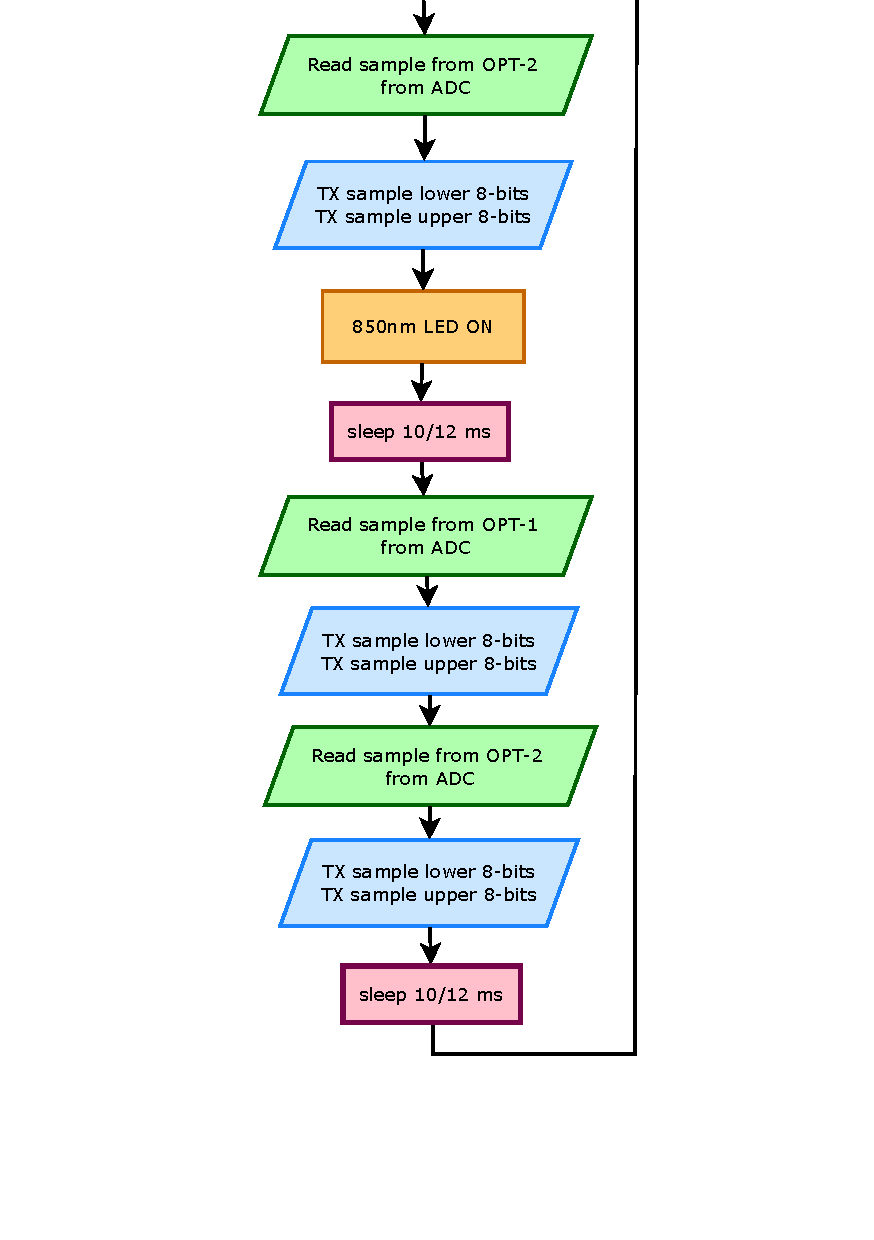
\includegraphics{cdia-3.pdf}
\end{figure}

\begin{figure}[htp]
\centering
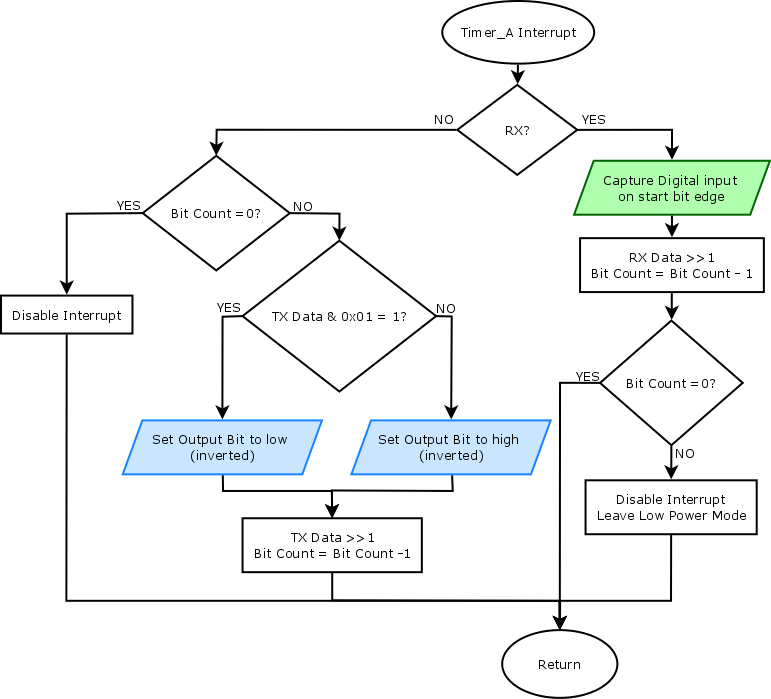
\includegraphics[width=6in]{cdiatimer.png}
\caption{Timer\_A interrupt flow chart}
\end{figure}

\headsep = 0.5in

\chapter {Matlab Source Code}
\lstinputlisting[language=Matlab,breaklines=true]{filter.m}